%% Spoken Compound Notation --- anonymous TOCHI manuscript
%% Compile with: ./compile.sh
%%   or: TEXINPUTS=./sty:./: pdflatex -interaction=nonstopmode main
%% Requires the ACM acmart class (https://www.acm.org/publications/authors/submissions)
%% BasicTeX lacks Libertine; disable font expansion so Computer Modern still ships a PDF.
\PassOptionsToPackage{expansion=false}{microtype}
\documentclass[manuscript, review, anonymous]{acmart}
% BasicTeX has no EC bitmap PK fonts; Latin Modern is already installed and scalable.
\usepackage{lmodern}

\acmJournal{TOCHI}
\acmYear{2026}
\acmVolume{0}
\acmNumber{0}
\acmArticle{0}
\acmMonth{0}

\usepackage{booktabs}
\usepackage{graphicx}
\usepackage{tabularx}
\usepackage{array}
\usepackage{amsmath}
\usepackage{tikz}
\usetikzlibrary{arrows.meta,positioning,fit,calc}

%% Numbered citations, sequentially as they appear (TOCHI requirement)
\citestyle{acmnumeric}

\setcopyright{none}

\begin{CCSXML}
<ccs2012>
 <concept>
  <concept_id>10003120.10003121.10003124</concept_id>
  <concept_desc>Human-centered computing~Interaction techniques</concept_desc>
  <concept_significance>500</concept_significance>
 </concept>
 <concept>
  <concept_id>10003120.10003121.10003122.10003334</concept_id>
  <concept_desc>Human-centered computing~Text input</concept_desc>
  <concept_significance>500</concept_significance>
 </concept>
 <concept>
  <concept_id>10003120.10003121.10003128</concept_id>
  <concept_desc>Human-centered computing~Interaction design theory, concepts and paradigms</concept_desc>
  <concept_significance>300</concept_significance>
 </concept>
 <concept>
  <concept_id>10003120.10003121.1176075</concept_id>
  <concept_desc>Human-centered computing~Accessibility systems and tools</concept_desc>
  <concept_significance>300</concept_significance>
 </concept>
 <concept>
  <concept_id>10011007.10011006.10011008.10011009</concept_id>
  <concept_desc>Software and its engineering~General programming languages</concept_desc>
  <concept_significance>100</concept_significance>
 </concept>
</ccs2012>
\end{CCSXML}

\ccsdesc[500]{Human-centered computing~Interaction techniques}
\ccsdesc[500]{Human-centered computing~Text input}
\ccsdesc[300]{Human-centered computing~Interaction design theory, concepts and paradigms}
\ccsdesc[300]{Human-centered computing~Accessibility systems and tools}
\ccsdesc[100]{Software and its engineering~General programming languages}

\keywords{spoken notation, array programming, Sanskrit compounds, operators, programming by voice, mathematical notation, sonic interaction, sam{\=a}sa}

\title{Spoken Compound Notation: Using Sanskrit Sam{\=a}sa to Represent Mathematical Operators in Sound}

\begin{abstract}
Mathematical notation is a tool of thought, but its most compact operator systems are hard to type and harder to speak. Iverson showed that a small written lexicon of functions and operators can generate a large executable language. P{\=a}{\d{n}}inian compound formation (\textit{sam{\=a}sa}) does the same in words: two compatible stems become one pronounceable form whose constituency remains recoverable. This paper designs a spoken operator language in which Sanskrit stems name array-language primitives and licensed compounds name derived operators. The language is implemented as a hold-to-talk keyboard that maps a speaker-dependent vocalization onto a glyph. Satuluri and Kulkarni's compound generator is recast as an interaction architecture---conceptual input, type assignment, constituent order, and sandhi only at the end---so that sound is treated as notation rather than as a dictation channel for English. The resulting 119-glyph lexicon is analyzed against Iverson's properties of notation: economy, suggestivity, subordination of detail, and executability. A running prototype shows where whole-clip acoustic matching collapses distinctions that compounding keeps apart. The contribution is a design theory and working system for sonic mathematical notation, together with an evaluation protocol that takes stem composition, not isolated word recognition, as the primary HCI object.
\end{abstract}

\begin{document}

\maketitle

\section{Introduction}

A good notation does more than record a result. It shapes the next thought. Whitehead's remark, cited by Iverson in the lecture that gives this paper its problem, is still the standard: by relieving the brain of unnecessary work, a good notation ``sets it free to concentrate on more advanced problems''~\cite{Iverson1980Notation,Whitehead1911Math}. Boole made the stronger claim that language is ``an instrument of human reason, and not merely a medium for the expression of thought''~\cite{Boole1854Laws}. Iverson's contribution was to insist that the instrument can be \emph{executed}. Programming languages, he argued, supply the universality and lack of ambiguity that ordinary mathematical notation lacks; a notation that is both executable and mathematically terse can be used as a tool of thought rather than as a transcription of thought already finished~\cite{Iverson1980Notation,Iverson1962APL}.

The operator is the device that makes that terseness generative. An operator applies to a function, or to functions, and produces a related function~\cite{Iverson1979Operators}. The slash in APL is not ``sum.'' Applied to plus it yields sum; applied to times it yields product; applied to maximum it yields the largest element. A few primitives generate a family. The written form is suggestive: $+/$ invites $\times/$, and $+\backslash$ invites $\times\backslash$. Economy and suggestivity are the same fact seen from two sides~\cite{Iverson1980Notation}.

That fact has a cost at the interface. Array-language glyphs---$\rho$, $\phi$, $\ddot{\phantom{a}}$, $\ddot{\circ}$, $\tilde{\ddot{\phantom{a}}}$---were designed for a page and a specialized keyboard, not for a voice or a laptop. Programming-by-voice systems therefore do the obvious thing: they replace the glyph with an English phrase. ``Reduce first,'' ``outer product,'' ``grade down by.'' The phrase is speakable. It is also a paraphrase. It throws away the economy that made the notation a tool of thought, and it does not generate. Nothing about saying ``reduce'' suggests saying ``scan,'' and nothing about saying ``not'' and ``and'' produces ``nand'' except by lexical accident.

This paper takes a different spoken analog of the operator. Sanskrit is unusually explicit about how two stems become one word. A compound (\textit{sam{\=a}sa}) is a single word (\textit{ekapadam}) whose meaning is built from constituents; sandhi at the join makes the result pronounceable; the constituency remains recoverable~\cite{Satuluri2013Generation,Gillon2009Tagging,Joshi1968Samartha}. Compounds are binary, recursive, and optional. Formation is licensed by semantic compatibility (\textit{s{\=a}marthya}) and by the speaker's desire (\textit{vakt\d{r}-vivak{\d{s}}{\=a}}): the grammar permits a join, it does not force one~\cite{Satuluri2013Generation}. The Cambridge Grammar of the English Language uses the same P{\=a}{\d{n}}inian classification for English compounds, which is to say the classification is a theory of compact expression, not a local curiosity~\cite{Huddleston2002Cambridge}.

The design claim is that Iverson's operator and P{\=a}{\d{n}}ini's compound are the same kind of object. Both take a small lexicon and a short list of joins and produce a much larger set of derived forms. Both subordinate detail: case endings disappear, axes disappear, the intermediate function is not written down. Both are suggestive: a licensed pattern invites the next licensed pattern. A spoken notation that inherits both properties would let a person \emph{speak in operators} rather than dictate English names for symbols.

The language designed here assigns Sanskrit stems to array-language primitives and forms derived operators as licensed compounds, predominantly \textit{tatpuru{\d{s}}a} (endocentric, second constituent as head). The stem \textit{{\=a}di} (first) and the stem \textit{sa{\d{m}}k{\d{s}}epa} (reduce) join as \textit{{\=a}disa{\d{m}}k{\d{s}}epa} and type the reduce-first glyph; \textit{ni{\d{s}}edha} (not) and \textit{sa{\d{m}}yoga} (and) join as \textit{ni{\d{s}}edhasa{\d{m}}yoga} and type NAND. Order carries meaning, as it does in the classical examples: clay-pot is not pot-clay~\cite{Satuluri2013Generation}. The language is implemented in a hold-to-talk keyboard, called {\'S}abda in this paper, that teaches a speaker-dependent vocalization per form and types the corresponding glyph into a buffer or into another application. Recognition is currently atomic---one clip, one nearest neighbor---which is an honest description of the prototype and a design problem the later sections treat as evidence, not as a finished result.

The paper makes four contributions.

\begin{enumerate}
\item A design theory that maps Iverson's properties of notation onto P{\=a}{\d{n}}inian compound formation, treating sonic notation as a first-class HCI object rather than as a speech front-end for an existing written language.
\item A spoken operator language: a stem inventory, a set of licensed joins, and a 119-glyph lexicon aligned with a modern array dialect (functions, monadic operators, dyadic operators, syntax and literals).
\item A working hold-to-talk system that makes the language executable at the point of utterance.
\item An evaluation protocol that tests composition---learnability, confusability, and the speaking of short executable expressions---rather than isolated word recall.
\end{enumerate}

The paper does not report a completed user study. TOCHI's archival standard requires evidence; the protocol in Section~\ref{sec:eval} is written so that the study can be run without redesigning the contribution. What the prototype already shows is the collision that a compositional account predicts: two taught names that compounding keeps apart sit almost on top of each other in embedding space.

The rest of the paper proceeds as follows. Sections~\ref{sec:iverson} and~\ref{sec:samasa} state the two source ideas with the precision the design needs. Section~\ref{sec:related} situates the work in HCI. Section~\ref{sec:framework} states the mapping. Section~\ref{sec:language} presents the language. Section~\ref{sec:system} describes the system. Section~\ref{sec:examples} walks through spoken expressions. Section~\ref{sec:analysis} evaluates the language against Iverson's criteria. Section~\ref{sec:prototype} reports what the running recognizer does to the theory. Section~\ref{sec:eval} gives the study protocol. Section~\ref{sec:discussion} discusses implications and limits.

\section{Notation as a Tool of Thought}
\label{sec:iverson}

Iverson's 1979 Turing Award lecture, published in 1980, is not a paper about APL so much as a paper about what a notation must be if it is to be used for thinking~\cite{Iverson1980Notation}. He begins from a deficit in ordinary mathematical notation: it is not universal, and it must be reinterpreted by topic, by author, and even by immediate context. Programming languages repair that deficit. They are general-purpose, unambiguous, and executable. Executability lets a machine run an extensive experiment on an idea; lack of ambiguity lets a person run a precise thought experiment. Most programming languages, he argues, then throw the mathematical advantages away. They are not suggestive. They are not economical. They do not subordinate detail. The thesis of the lecture is that executability and mathematical terseness can occupy one language.

The characteristics he uses to shape the argument are five, in addition to executability and universality~\cite{Iverson1980Notation}:

\begin{description}
\item[Ease of expressing constructs arising in problems.] A notation must express not only the problem as first stated but the notions that appear when the problem is generalized, specialized, or taken apart.
\item[Suggestivity.] The form of an expression arising in one problem should suggest related expressions that apply in others.
\item[Subordination of detail.] Brevity facilitates reasoning. Brevity is achieved by arrays, by names, and by operators.
\item[Economy.] A large number of ideas must be expressible from a small vocabulary and simple grammatical rules.
\item[Amenability to formal proofs.] Identities should be writable in a form that is itself an object of calculation.
\end{description}

The running example is the close-packed crystal. The numbers of atoms in successive rows are $\iota 5$; their sum is $+/\,\iota 5$; the partial sums are $+\backslash\,\iota 5$; the tetrahedron they generate is $+/+\backslash\,\iota 5$. Each step is a reuse of a form that the previous step made visible. Suggestivity is operational: the notation produces the next question.

The operator is how the language stays small while that reuse goes on. Iverson defines an operator as an object that applies to a function or functions and produces a related function~\cite{Iverson1979Operators}. Familiar mathematical operators---derivative, tensor product, composition, Laplace and Fourier transforms---already work this way. APL makes three of them primitive and everyday: reduction ($/ $), scan ($\backslash$), and inner product ($.$). Reduction applied to plus is summation; applied to times is the product commonly written $\Pi$; applied to and, or, maximum, and minimum it produces the corresponding folds. The point is not the particular glyphs. The point is that the slash is a generator. ``Because a small number of functions and operators can be combined to produce a much larger set of derived functions, the use of operators can lead to great economy in the number of distinct functions required, and also to the recognition of structure in the set of functions employed''~\cite{Iverson1979Operators}.

Two syntactic facts from that paper matter for a spoken design. First, a monadic function applies to its right, while a monadic operator applies to its left: operators and functions are mirror images. Second, a derived function may itself be the argument of an operator. The language is recursive in the same sense that a compound's constituent may itself be a compound.

Iverson also insists that notation suited as a tool of thought should be introducible \emph{in context}, the way mathematical notation is introduced, and not taught as a separate course the way programming languages commonly are~\cite{Iverson1980Notation}. A spoken design that requires a person to memorize 119 unrelated names before writing $\iota 5$ has already failed that test. A design that lets a person learn \textit{sa{\d{m}}k{\d{s}}epa} and then discover \textit{{\=a}disa{\d{m}}k{\d{s}}epa} in the same session has not.

The lecture is not an interface paper. It has nothing to say about keyboards, voices, or who can use the notation. That is the HCI remainder. If operators are the reason the written language thinks well, then an interface that cannot say an operator---or that can say it only by abandoning the operator for an English paraphrase---is not a transparent channel. It is a different notation, and a worse one by Iverson's own criteria.

\section{Sanskrit Compound Formation as a Generative Notation}
\label{sec:samasa}

Satuluri and Kulkarni rewrite P{\=a}{\d{n}}ini's compound rules as a generator~\cite{Satuluri2013Generation}. The paper is the second source of this design, and it is important to say what it is not. It is not a theory of speech sounds as symbols. It is not an acoustic model. It is a computational account of how two stems become one written word, with sandhi as a late, obligatory pronunciation step. That is exactly the structure a spoken operator language needs: meaning and type first, sound last.

\subsection{Why compounds exist}

Compounds, they write, ``provide a compact way of expressing the thoughts.'' They bring brevity, and they enrich the language at both the lexical and the structural level~\cite{Satuluri2013Generation}. For a language rich in compounds, analysis and generation are not optional decorations on a parser; they are how the language makes new words. Indian grammatical tradition discusses compounds at two levels: \textit{prakriy{\=a}}, the morphophonological formation, and \textit{artha}, the meaning. The \textit{samarth{\=a}hnika} of Pata{\~n}jali, as edited by Joshi, is the classical discussion of semantic compatibility and of the compositionality of a compound's meaning from its parts~\cite{Joshi1968Samartha}. Mahavir and Murti treat the same process as a philosophical and grammatical object~\cite{Mahavir1986Samasa,Murti1974Compounds}.

Two structural facts are used throughout the present paper. Compounds are binary, with the exception of coordinative (\textit{dvandva}) compounds and some exocentric (\textit{bahuvr{\=\i}hi}) compounds. Individual components may themselves be compounds, so formation is recursive, and the constituency structure is what makes a nested compound understandable~\cite{Gillon2009Tagging,Satuluri2013Generation}. A notation that erases constituency---for example by embedding a whole compound as one acoustic vector---has thrown away the thing the grammar is for.

\subsection{Four types}

P{\=a}{\d{n}}ini's semantic classification is the working typology. Huddleston and Pullum use it for English, which is the authors' own warrant that the types are a general account of compact naming~\cite{Huddleston2002Cambridge,Satuluri2013Generation}.

\begin{description}
\item[Tatpuru{\d{s}}a] (endocentric). The second constituent is the head. \textit{r{\=a}japuru{\d{s}}a{\d{h}}} is a man, of a king. Most derived operators in the language designed here are tatpuru{\d{s}}a: the operator is the head, the modifier restricts it.
\item[Avyay{\=\i}bh{\=a}va.] The first constituent is the head. The result is an indeclinable, always neuter. \textit{upak{\d{r}}{\d{s}}{\d{n}}am} is ``near K{\d{r}}{\d{s}}{\d{n}}a,'' and the new stem does not take further case. In a spoken operator language this is the type of a closed form: a finished adverbial or prefixal operator that is not offered for further compounding in the same breath.
\item[Bahuvr{\=\i}hi] (exocentric). The compound is an adjective whose head is outside it. \textit{p{\=\i}t{\=a}mbara{\d{h}}} is not a cloth and not the color yellow; it is the one whose cloth is yellow. Some operator names in the lexicon are bahuvr{\=\i}hi in spirit: they name a derived function by a property rather than by a head operation.
\item[Dvandva] (coordinative). Both constituents are heads. \textit{r{\=a}mak{\d{r}}{\d{s}}{\d{n}}au} is Rama and Krishna. The spoken analog is a coordinated pair of operators, or two glyphs spoken as one word with dual or plural result.
\end{description}

Order is meaning. \textit{m{\d{r}}ttik{\=a}gha{\d{t}}a{\d{h}}} is a pot made of clay; \textit{gha{\d{t}}am{\d{r}}ttik{\=a}} is the clay for a pot~\cite{Satuluri2013Generation}. A recognizer that treats a clip as a bag of stems will identify those two forms. A notation that claims to be a tool of thought cannot.

\subsection{The derivation as a pipeline}

Satuluri and Kulkarni collect some four hundred s{\=u}tras of the A{\d{s}}{\d{t}}{\=a}dhy{\=a}y{\=\i} that deal with compounding and split them into two machines~\cite{Satuluri2013Generation}. \textit{Sa{\d{m}}j{\~n}{\=a}} s{\=u}tras assign a technical label to a string or a part of it (\textit{sam{\=a}sa}, \textit{upasarjana}, \textit{pr{\=a}tipadika}, type). They are implemented as a context-free grammar. \textit{Vidhi} s{\=u}tras transform the string. They are implemented as a regular grammar with three rewrite shapes:

\begin{align}
W_1\,W_2 &\rightarrow W_3\,W_2 && \text{left changes in the context of the right} \label{eq:rightctx}\\
W_1\,W_2 &\rightarrow W_1\,W_3 && \text{right changes in the context of the left} \label{eq:leftctx}\\
W_1\,W_2 &\rightarrow W_1\,W_2\,W_3 && \text{a suffix is appended} \label{eq:append}
\end{align}

Labels create an environment; processes fire inside it. That is already the operator: the slash is not a function, it is a label that turns plus into sum.

The tradition's procedure, as they reconstruct it, is a sequence of named stages. The input is not the surface sentence. It is an \textit{alaukika vigraha}, a conceptual paraphrase in which stems carry explicit case markers: \textit{r{\=a}jan + {\.n}as puru{\d{s}}a + su} for ``king's man.'' The governing s{\=u}tra is \textit{samartha{\d{h}} padavidhi{\d{h}}} (P2.1.1). A compound forms only if the meanings are compatible, and only if the speaker wants the compact form. The paraphrase is then labeled a \textit{sam{\=a}sa}. Optional \textit{sam{\=a}s{\=a}nta} suffixes may be added. The constituent that will occupy first position is labeled \textit{upasarjana} and moved there (\textit{p{\=u}rvanip{\=a}ta}). The whole string is declared a nominal stem. Case suffixes are elided (\textit{subluk}), except in listed cases (\textit{aluk}). Each stem may change in the presence of the other. Obligatory stem-final operations apply. Then, and only then, the two stems are joined by sandhi: \textit{r{\=a}ma + {\=a}laya $\rightarrow$ r{\=a}m{\=a}laya}. Gender and number of the new stem are assigned by type. Word formation produces the usable word.

Sandhi is step eleven of thirteen. The phonetics of the join are not the theory of the compound. They are how the already-decided compound is said. This is the fact most easy to miss if one hears ``the compounding nature of Sanskrit sounds'' as an acoustic claim. In the source paper, sounds compound after the operator structure is fixed.

\subsection{What the generator needs besides the string}

Some s{\=u}tras consult information that is not in the phoneme sequence: morphological analysis, ontological category, lexical meaning, and the relation between the two components~\cite{Satuluri2013Generation}. The relations they implement include part--whole, comparison, and opposition. \textit{{\'s}{\=\i}ta} and \textit{u{\d{s}}{\d{n}}a} (cold and hot) are licensed as a pair because they are opposed. A spoken operator language needs the same kind of filter. Not every pair of stems is an operator. \textit{ni{\d{s}}edha} and \textit{sa{\d{m}}yoga} are licensed (NAND). \textit{viloma} and \textit{{\=a}k{\=a}ra} are not. The lexicon of allowed joins \emph{is} the grammar.

Computational work around the generator---constituency parsing~\cite{Kulkarni2011Parser}, compound processors~\cite{Kumar2010Processor}, type identification that mixes grammar and corpus~\cite{Krishna2016Compound}, and Huet and Goyal's morphological platforms~\cite{Huet2009Formal,Goyal2013Reader}---establishes that the formation is precise enough to run. Kadvany's reading of P{\=a}{\d{n}}ini as a generative computational language is the broader warrant for treating the grammar as a designed formal system rather than as heritage decoration~\cite{Kadvany2014Panini}. The present paper does not implement four hundred s{\=u}tras. It takes the generator's architecture---labels, context-sensitive rewrites, late sandhi, optional formation---and uses it as an interaction architecture for operators in sound.

\section{Related Work}
\label{sec:related}

The work sits at the intersection of programming-by-voice, mathematical accessibility, the psychology of notations, and sonic interaction. Each literature has a gap that the others do not fill.

\subsection{Programming by voice}

Programming languages are not meant to be spoken. D{\'e}silets stated the usability problems clearly for VoiceGrip and VoiceCode: punctuation is dense, identifiers are irregular, and homophony is constant~\cite{Desilets2001VoiceGrip,Desilets2006VoiceCode}. The productive response in that line of work is a speakable \emph{pseudo-syntax} that a translator then renders into the native language. Arnold, Mark, and Goldthwaite's VocalProgramming, Wagner and Gray's vocal UI, and Rosenblatt and colleagues' VocalIDE extend the same idea toward people with motor impairments, with demonstrated gains for navigation and selection~\cite{Arnold2000VocalProgramming,Wagner2015Vocal,RosenblattVocalIDE}. Commercial and community systems such as Talon continue the approach: English-like commands, heavy customization, a long learning tail.

The present work shares the accessibility motive and the hold-to-talk phrase structure. It rejects the premise that the spoken form should be a pseudo-English for an unchanged written language. VoiceCode makes Java speakable by adding a layer. An operator language makes the spoken form itself the notation. The distinction matters for Iverson's criteria. A pseudo-syntax that expands every glyph into a multi-word English command improves utterability and destroys economy. A compound stem language keeps the generative rule.

Ability-based design is the right framing for the accessibility claim~\cite{Wobbrock2011Ability}. The system should be usable without a keyboard; it should not assume that the interesting user is a disabled exception to a keyboard default. Feng and Sears's work on confidence-aware speech navigation in TOCHI is the closest archival precedent for treating recognition uncertainty as part of the interaction, not as an engineering remainder~\cite{Feng2004TOCHI}. The prototype's cosine threshold is a crude version of that idea and is called out as such in Section~\ref{sec:prototype}.

\subsection{Speaking mathematics}

Mathematical accessibility has a mature spoken notation: Nemeth Braille, Raman's AsTeR, MathPlayer, and later ClearSpeak-style speech rules for MathML~\cite{Nemeth1972Math,Raman1994AsTeR,Soiffer2005ASSETS,Sorge2014W4A,Baartse2018ClearSpeak}. That literature is about \emph{reading} existing written mathematics aloud with enough structure that a listener can recover nesting. It is not about \emph{writing} an executable operator language by speaking it. The two problems share a requirement---constituency must survive the acoustic channel---and they do not share a solution. A screen reader that says ``the sum from $i$ equals one to $n$ of $x$ sub $i$'' is a paraphrase of $\sum$. It is a good paraphrase. It is not $+/x$, and it does not suggest $\times/x$.

\subsection{Notations as cognitive artifacts}

Green's cognitive dimensions, and Green and Petre's application of them to visual programming, give HCI a vocabulary for talking about notations without reducing them to visual style~\cite{Green1989Design,Green1996Cognitive}. Closeness of mapping, hidden dependencies, viscosity, role-expressiveness, and premature commitment are all live for a spoken operator language. Iverson's suggestivity is close to role-expressiveness plus closeness of mapping; his subordination of detail is a deliberate increase in hidden dependency in exchange for a drop in viscosity. The present analysis uses Iverson's terms because they are native to the operator, and uses cognitive dimensions when an interface property (error recovery, progressive evaluation, hard mental operations) is not in Iverson's list.

Norman and Zhang treat external representations as cognitive artifacts that change what a person can think~\cite{Norman1991Artifacts,Zhang1994Representations}. Hutchins's distributed account is the social and material version of the same claim~\cite{Hutchins1995Cognition,Hutchins1995Distributed}. A spoken operator is an artifact in that sense: it is not a command issued to a tool, it is a representation the tool and the speaker share. Beaudouin-Lafon's instrumental interaction and Jacob and colleagues' reality-based interaction both argue for post-WIMP instruments that have a graspable domain analog~\cite{Beaudouin2000CHI,Jacob2008CHI}. Voice is a poor analog of a glyph and a good analog of a word. The design takes that seriously.

Olsen's UIST argument about evaluating interface systems research is the methodological constraint~\cite{Olsen2007UIST}. A new notation cannot be evaluated only by comparing task times against QWERTY on a task the old notation already owns. The evaluation has to ask whether the new representation makes a previously awkward class of thought available. Section~\ref{sec:eval} is written to that standard.

\subsection{Sonic interaction and speech interfaces}

Earcons have internal structure: they were designed, from the beginning, as a compositional auditory language~\cite{Blattner1989Earcons}. Sonic interaction design treats sound as a medium of manipulation, not only of display~\cite{Franinovic2013Sonic}. Speech user interfaces, from SpeechActs forward, have warned that speakable English is not the same as a well-designed spoken language~\cite{Yankelovich1995CHI,Pearl2016VUI,Corbett2016VUIs}. The present work is closer to earcons than to conversational agents. The user is not talking to an assistant about a program. The user is speaking the program.

Harada's vocal joystick showed that continuous voice can be an analog instrument~\cite{Harada2006Joystick}. {\'S}abda is discrete: a held key delimits a phrase, as Buxton argued chunking and phrasing should~\cite{Buxton1986Chunking}. The hold-to-talk key is the phrasing device.

\subsection{Language, colonialism, and who gets to name operators}

Using Sanskrit in an HCI system is not a neutral aesthetic choice. Irani and colleagues' postcolonial computing is the required caution~\cite{Irani2010CHI}. Sanskrit has been mobilized as cultural supremacy as often as it has been studied as a formal system. The warrant for using it here is specific and narrow: it has an explicit, implemented theory of compact generative naming that English operator-paraphrase does not. The stems are IAST and are taught as a designed lexicon, not as a test of heritage knowledge. The evaluation protocol includes speakers with and without prior Sanskrit, and treats prior knowledge as a covariate, not as a prerequisite. That does not finish the political problem. It is the minimum that makes the design honest.

\section{Design Framework: Operators as Compounds}
\label{sec:framework}

The mapping is stated as a correspondence, then as an interaction architecture.

\subsection{The correspondence}

Table~\ref{tab:map} is the design in one place.

\begin{table}[t]
\caption{Correspondence between Iverson's operators and P{\=a}{\d{n}}inian compounds. The spoken language is the image of the left column under the right.}
\label{tab:map}
\begin{tabular}{p{0.30\columnwidth}p{0.30\columnwidth}p{0.30\columnwidth}}
\toprule
\textbf{Iverson} & \textbf{Sam{\=a}sa} & \textbf{Spoken design} \\
\midrule
Function ($+$, $\times$) & Stem (\textit{yugma}, \textit{gu{\d{n}}ana}) & Taught vocalization of a stem \\
Operator ($/$, $\backslash$, $.$) & Compound type and join & Licensed stem pair \\
Derived function ($+/$) & Surface compound (\textit{{\=a}disa{\d{m}}k{\d{s}}epa}) & Spoken compound or sequential stems \\
Monadic operator applies left & \textit{Upasarjana} / order & First stem is the modifier when type is tatpuru{\d{s}}a \\
Operator on a derived function & Recursive compound & A compound as a constituent \\
Suggestivity of $+/$ to $\times/$ & Same head, new modifier & Same head stem, new left stem \\
Optional use of an operator & \textit{Vivak{\d{s}}{\=a}} & Speaker may say the paraphrase instead \\
Well-formed expression & \textit{S{\=a}marthya} & Only licensed joins type a glyph \\
Spelling / sandhi of a written word & Sandhi as last step & Pronunciation of an already-typed join \\
\bottomrule
\end{tabular}
\end{table}

Iverson's rewrite shapes and Satuluri and Kulkarni's vidhi shapes are the same family. Equation~\ref{eq:rightctx} is the monadic operator: the left function changes in the context of the operator on its right, if one writes the spoken sequence modifier-then-head, or the operator changes the function on its left, if one writes the APL sequence function-then-operator. The present language adopts modifier-then-head, the tatpuru{\d{s}}a default, because that is how the Sanskrit names in the lexicon are already formed and because it matches English modifier order (``first-reduce'') without matching English verbosity.

\subsection{An interaction architecture}

The generator's stages become turns in an interface (Figure~\ref{fig:pipeline}).

\begin{figure}[t]
\centering
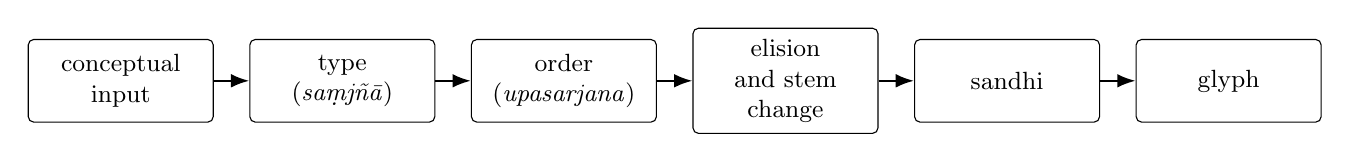
\begin{tikzpicture}[
  node distance=0.45cm,
  box/.style={draw, rounded corners=2pt, align=center, inner sep=4pt, font=\small,
              minimum width=2.35cm, minimum height=1.05cm},
  arr/.style={-{Latex}, thick}
]
\node[box] (a) {conceptual\\input};
\node[box, right=of a] (b) {type\\(\textit{sa{\d{m}}j{\~n}{\=a}})};
\node[box, right=of b] (c) {order\\(\textit{upasarjana})};
\node[box, right=of c] (d) {elision\\and stem\\change};
\node[box, right=of d] (e) {sandhi};
\node[box, right=of e] (f) {glyph};
\draw[arr] (a) -- (b);
\draw[arr] (b) -- (c);
\draw[arr] (c) -- (d);
\draw[arr] (d) -- (e);
\draw[arr] (e) -- (f);
\end{tikzpicture}
\caption{Satuluri and Kulkarni's compound pipeline, read as an interaction architecture. Type and order are decided before sound fuses. The current prototype jumps from conceptual input to glyph by nearest-neighbor embedding; the missing middle is the research object.}
\label{fig:pipeline}
\end{figure}

\begin{description}
\item[Conceptual input.] The speaker intends an operator, not a waveform. The interface's job is to recover stems and a type, not to classify a clip against 119 exemplars.
\item[Type assignment.] A label---tatpuru{\d{s}}a, avyay{\=\i}bh{\=a}va, bahuvr{\=\i}hi, dvandva, or simplex stem---selects which rewrite applies. The label is the operator.
\item[Order.] \textit{{\=a}di} then \textit{sa{\d{m}}k{\d{s}}epa} is reduce-first. The reverse is not a defined join. The interface must not be commutative unless the type is dvandva.
\item[Elision.] Spoken case and English articles never enter the stem channel. ``The first reduce'' and \textit{{\=a}di sa{\d{m}}k{\d{s}}epa} are the same conceptual input.
\item[Sandhi.] If the speaker produces the fused word \textit{{\=a}disa{\d{m}}k{\d{s}}epa}, that is a pronunciation of a join already licensed, not a third primitive.
\item[Glyph.] The executable mark. Typing it is Iverson's executability, at the scale of a keystroke.
\end{description}

Two paths are first-class, corresponding to \textit{vivak{\d{s}}{\=a}}. A fluent speaker says the compound. A novice says the stems in order, or says an English paraphrase that the interface treats as a vigraha and compiles to the same glyph. Iverson's ``introduction in context'' is this optionality~\cite{Iverson1980Notation}. The grammar allows the compact form; it does not require it on the first encounter.

\subsection{What would falsify the mapping}

If speakers cannot recover a new licensed compound from known stems at a rate above a memorized-name control, suggestivity has failed. If stem-then-stem recognition does not beat whole-clip recognition on near pairs, the pipeline's claim that type-before-sandhi matters acoustically has failed. If licensed-join constraints do not reduce false glyphs relative to an open 119-way classifier, \textit{s{\=a}marthya} is ornamental. The evaluation protocol is built from those falsifiers.

\section{The Spoken Operator Language}
\label{sec:language}

The language is a stem inventory, a join grammar, and a glyph table. It is designed, not harvested. Where a classical word already named the operation, that word is kept. Where array programming needed a name that Sanskrit does not lexicalize as a single everyday stem, a tatpuru{\d{s}}a was formed and checked against the naming conventions in Table~\ref{tab:conventions}.

\subsection{Naming conventions}

\begin{table}[t]
\caption{Recurring stems that generate families, rather than isolated translations.}
\label{tab:conventions}
\begin{tabular}{lll}
\toprule
\textbf{Devan{\=a}gar{\=\i}} & \textbf{IAST} & \textbf{Role in the language} \\
\midrule
kriy\=a & \textit{kriy{\=a}} & a process; used in operator names \\
sa\d{m}yojana & \textit{sa{\d{m}}yojana} & composition of functions \\
sth\=ana & \textit{sth{\=a}na} & position, index, where \\
ga\d{n}an\=a & \textit{ga{\d{n}}an{\=a}} & counting, tally \\
vibh\=ajana & \textit{vibh{\=a}jana} & split, drop \\
viloma & \textit{viloma} & reverse, invert \\
ak\d{s}a & \textit{ak{\d{s}}a} & array axis \\
m\=ula & \textit{m{\=u}la} & root, foundational operation \\
\=adi & \textit{{\=a}di} & first axis, first constituent \\
ni\d{s}edha & \textit{ni{\d{s}}edha} & logical not, without \\
sama & \textit{sama} & equality, the ``also-equal'' close \\
\bottomrule
\end{tabular}
\end{table}

Devan{\=a}gar{\=\i} in Table~\ref{tab:conventions} is a written reminder, not an input requirement. Speakers train and use IAST. The point of the table is economy: \textit{{\=a}di} is not a word for one glyph. It is a modifier that generates a family.

\subsection{Stem inventory}

Table~\ref{tab:stems} lists the productive stems. Simplex glyphs that do not (yet) participate in joins---\textit{v{\d{r}}tta} for circular functions, \textit{p{\=a}{\'s}a} for roll---are in the full lexicon (Appendix~\ref{app:lexicon}) and are treated as frozen lexemes, analogously to Iverson's primitive functions that have not been fed to an operator.

\begin{table}[t]
\caption{Productive stems. A speaker who knows this list can generate the derived operators in Table~\ref{tab:joins} without a new memorized word.}
\label{tab:stems}
\begin{tabular}{lll}
\toprule
\textbf{Stem} & \textbf{Gloss} & \textbf{Simplex glyph, if any} \\
\midrule
\textit{yugma} & pair, join, add & $+$ \\
\textit{viyoga} & separation, subtract, nor-part & $-$ \\
\textit{gu{\d{n}}ana} & multiply & $\times$ \\
\textit{bh{\=a}ga} & divide, share & $\div$ \\
\textit{ni{\d{s}}edha} & not, without & $\sim$ \\
\textit{sa{\d{m}}yoga} & conjunction, and & (head in NAND) \\
\textit{sama} / \textit{samat{\=a}} & equal & $=$ \\
\textit{ny{\=u}na} & less & $<$ \\
\textit{adhika} & greater & $>$ \\
\textit{sa{\d{m}}k{\d{s}}epa} & reduce & $/$ \\
\textit{sa{\d{m}}caya} & scan & $\backslash$ \\
\textit{viloma} & reverse, invert & reverse / rotate \\
\textit{graha{\d{n}}a} & take, first & (head in take) \\
\textit{{\=a}di} & first (axis) & --- \\
\textit{{\=a}k{\=a}ra} & shape & $\rho$ \\
\textit{sth{\=a}na} & where, place & where \\
\textit{v{\=a}ma} & left & left / same-left \\
\textit{dak{\d{s}}i{\d{n}}a} & right & right / same \\
\textit{tarka} & argument & (in $\alpha$, $\omega$) \\
\textit{s{\=a}dhana} & operand & (in $\alpha$, $\omega$ operands) \\
\textit{p{\=u}rva} & before & (in bind-left) \\
\textit{uttara} & after & (in bind-right) \\
\textit{bandha} & bind & (head of binds) \\
\textit{sa{\d{m}}yojana} & compose, atop & $\circ$ \\
\textit{kriy{\=a}} & operation & (in under, recursion) \\
\textit{punar} & again & (in power, recursion) \\
\textit{{\=a}v{\d{r}}tti} / \textit{{\=a}vartana} & iteration, recursion & power, recursion \\
\textit{krama} & sequence & (in factorial) \\
\textit{bahis} / \textit{bahir} & outer & (in outer product) \\
\textit{a-} & privative prefix & (in $\neq$, \textit{asamat{\=a}}) \\
\bottomrule
\end{tabular}
\end{table}

\subsection{Licensed joins}

Table~\ref{tab:joins} is the grammar that Satuluri and Kulkarni would call the s{\=u}tras that ``guarantee the formation''~\cite{Satuluri2013Generation}. The default type is tatpuru{\d{s}}a: $W_1 W_2 \rightarrow W_1W_2$ with $W_2$ as head. Sandhi is written in the surface column; the conceptual input is the pair of stems.

\begin{table}[t]
\caption{Licensed tatpuru{\d{s}}a joins. Head is the second stem. Surface forms already appear on the system's tiles; the contribution is to treat them as generated, not as captions.}
\label{tab:joins}
\begin{tabular}{llll}
\toprule
\textbf{Stems} & \textbf{Surface} & \textbf{Glyph} & \textbf{Meaning} \\
\midrule
\textit{{\=a}di} $+$ \textit{sa{\d{m}}k{\d{s}}epa} & \textit{{\=a}disa{\d{m}}k{\d{s}}epa} & reduce-first & reduce along first axis \\
\textit{{\=a}di} $+$ \textit{sa{\d{m}}caya} & \textit{{\=a}disa{\d{m}}caya} & scan-first & scan along first axis \\
\textit{{\=a}di} $+$ \textit{viloma} & \textit{{\=a}diviloma} & reverse-first & reverse / rotate first axis \\
\textit{{\=a}di} $+$ \textit{graha{\d{n}}a} & \textit{{\=a}digraha{\d{n}}a} & take & first / take \\
\textit{ni{\d{s}}edha} $+$ \textit{sa{\d{m}}yoga} & \textit{ni{\d{s}}edhasa{\d{m}}yoga} & NAND & not-and \\
\textit{ni{\d{s}}edha} $+$ \textit{viyoga} & \textit{ni{\d{s}}edhaviyoga} & NOR & not-or \\
\textit{ny{\=u}na} $+$ \textit{sama} & \textit{ny{\=u}nasama} & $\leq$ & less-or-equal \\
\textit{adhika} $+$ \textit{sama} & \textit{adhikasama} & $\geq$ & greater-or-equal \\
\textit{a-} $+$ \textit{samat{\=a}} & \textit{asamat{\=a}} & $\neq$ & not-equal \\
\textit{krama} $+$ \textit{gu{\d{n}}ita} & \textit{krama-gu{\d{n}}ita} & $!$ & factorial \\
\textit{bahir} $+$ \textit{gu{\d{n}}ana} & \textit{bahirgu{\d{n}}ana} & outer & outer product \\
\textit{p{\=u}rva} $+$ \textit{bandha} & \textit{p{\=u}rvabandha} & bind-left & before / bind left \\
\textit{uttara} $+$ \textit{bandha} & \textit{uttarabandha} & bind-right & after / bind right \\
\textit{v{\=a}ma} $+$ \textit{tarka} & \textit{v{\=a}matarka} & left-arg & left argument \\
\textit{dak{\d{s}}i{\d{n}}a} $+$ \textit{tarka} & \textit{dak{\d{s}}i{\d{n}}atarka} & right-arg & right argument \\
\textit{v{\=a}ma} $+$ \textit{s{\=a}dhana} & \textit{v{\=a}mas{\=a}dhana} & left-op & left operand \\
\textit{dak{\d{s}}i{\d{n}}a} $+$ \textit{s{\=a}dhana} & \textit{dak{\d{s}}i{\d{n}}as{\=a}dhana} & right-op & right operand \\
\textit{adhi} $+$ \textit{sa{\d{m}}yojana} & \textit{adhisa{\d{m}}yojana} & atop & function composition \\
\textit{adhas} $+$ \textit{kriy{\=a}} & \textit{adha{\d{h}}kriy{\=a}} & under & under \\
\textit{punar} $+$ \textit{{\=a}v{\d{r}}tti} & \textit{punar{\=a}v{\d{r}}tti} & power & power / iteration \\
\textit{punar} $+$ \textit{{\=a}vartana} & \textit{punar{\=a}vartana} & recursion & recursion \\
\textit{punar{\=a}vartana} $+$ \textit{kriy{\=a}} & \textit{punar{\=a}vartanakriy{\=a}} & op-rec & operator recursion \\
\textit{m{\=a}tr{\=a}} $+$ \textit{viloma} & \textit{m{\=a}tr{\=a}viloma} & mat-inv & matrix inverse \\
\textit{ku{\~n}j{\=\i}} $+$ \textit{kara{\d{n}}a} & \textit{ku{\~n}j{\=\i}kara{\d{n}}a} & key & key operator \\
\textit{sva} $+$ \textit{parivartana} & \textit{svaparivartana} & commute & self / commute \\
\textit{prati} $+$ \textit{eka} & \textit{pratyeka} & each & each \\
\textit{prati} $+$ \textit{r{\=u}pa} & \textit{pratir{\=u}pa} & stencil & stencil \\
\textit{samuccaya} $+$ \textit{ko{\d{s}}{\d{t}}haka} & \textit{samuccayako{\d{s}}{\d{t}}haka} & $[\,]$ & array brackets \\
\textit{pada} $+$ \textit{vibh{\=a}jaka} & \textit{padavibh{\=a}jaka} & token-sep & token separator \\
\textit{do{\d{s}}a} $+$ \textit{rak{\d{s}}aka} & \textit{do{\d{s}}arak{\d{s}}aka} & $::$ & error guard \\
\textit{g{\d{r}}h{\=\i}ta} $+$ \textit{do{\d{s}}a} & \textit{g{\d{r}}h{\=\i}tado{\d{s}}a} & error & caught error \\
\bottomrule
\end{tabular}
\end{table}

The table is not exhaustive of the 119 glyphs; it is exhaustive of the claim. If a name does not decompose, it is a primitive. If it does, a speaker who knows the parts should be able to produce or recognize the join on the first encounter. That is Iverson's suggestivity, stated as a test.

\subsection{Grammar}

A fragment, in the style of Satuluri and Kulkarni's Table~2~\cite{Satuluri2013Generation}:

\begin{quote}
\small
\textit{utterance} ::= \textit{stem} $\mid$ \textit{sam{\=a}sa} $\mid$ \textit{vigraha}\\
\textit{sam{\=a}sa} ::= \textit{stem} \textit{stem}  \quad\textit{\{ if licensed(type, stem$_1$, stem$_2$) \}}\\
\textit{vigraha} ::= English or IAST paraphrase compiling to the same glyph\\
\textit{type} ::= tatpuru{\d{s}}a $\mid$ avyay{\=\i}bh{\=a}va $\mid$ bahuvr{\=\i}hi $\mid$ dvandva $\mid$ simplex\\
\textit{action} ::= assign-type; order; elide; sandhi-optional; emit-glyph
\end{quote}

\textit{licensed} is the finite relation in Table~\ref{tab:joins} plus the simplex rows of the full lexicon. An unlicensed pair is a recognition failure, not a guess. That is stricter than the current prototype and is the intended system.

\subsection{Why Sanskrit, and why not English compounds}

English already compounds (``first-reduce,'' ``left-bind''). The Cambridge Grammar's use of the P{\=a}{\d{n}}inian types is an argument that the \emph{types} are available in English~\cite{Huddleston2002Cambridge}. English is still a poor operator language for three reasons the design cares about. First, English operator-paraphrase is long: ``reduce along the first axis'' is a clause, not a stem. Second, English compounds are orthographically unstable (spaces, hyphens, fusion) and phonologically weak: ``first reduce'' and ``reduce first'' are easy to swap, and the language does not mark the swap as a change of type. Third, English already owns the dictation channel. Using it reimports the VoiceCode solution the paper is trying not to take.

Sanskrit stems are short, stress-light, and already equipped with an implemented join rule and a mandatory sandhi story. IAST keeps them writable on a Latin keyboard and speakable by a non-reader of Devan{\=a}gar{\=\i}. The language is a designed dialect, not a claim that array programmers should learn classical Sanskrit.

\section{The {\'S}abda System}
\label{sec:system}

{\'S}abda is a speaker-dependent, few-shot spoken keyboard for the lexicon. It is a research system, not a product evaluation. This section describes what is implemented, so that the gap in Figure~\ref{fig:pipeline} is concrete.

\subsection{Interface}

Two views share a session. \emph{Sound Names} presents the 119 glyphs in four families---functions (61), monadic operators (11), dyadic operators (12), syntax and literals (35). Each tile shows an English gloss, the glyph, and the IAST name. Selecting an untaught tile starts a short recording; the clip is stored as an example of that name. \emph{Sound Keyboard} is the executable view. The user turns the keyboard on, holds a modifier (Right Option, Right Command, or Right Control), produces a sound, and releases. The matching glyph is inserted into an on-page buffer, or, with permission, into the frontmost application. A hold-to-talk button duplicates the modifier for use without a physical key. A treemap of taught sounds, sized by number of examples, sits under the keyboard as a library, not as a command menu.

The hold key is Buxton's phrase delimiter~\cite{Buxton1986Chunking}. A web page cannot see keys when it is in the background and cannot type into other applications; the desktop host therefore watches the chosen modifier system-wide and posts Unicode when ``use in other apps'' is on. That engineering is in service of executability: an operator that cannot leave the demo page is not Iverson's operator.

\subsection{Recognition}

Audio is 16\,kHz PCM from the browser, trimmed of quiet lead-in and tail so that wait time does not become part of the name. A wav2vec~2.0 base model~\cite{Baevski2020Wav2vec}, run locally, produces frame-level hidden states. The embedding is the mean of the real frames (padding is dropped), minus a fixed ``typical audio'' center, then L2-normalized to 768 dimensions. Each taught name stores up to a dozen such vectors. A new clip is scored by the maximum cosine similarity to any stored vector of each name. Scores are sharpened with a softmax at temperature $1/40$ so that a crowded top can be displayed as a distribution. A name is accepted only if the best cosine is at least $0.6$; otherwise the interface reports that it is not sure and shows the nearest neighbors.

The threshold is empirical and local. Informal self-use on the prototype found same-name repeats centering near $0.82$ (with a long tail) and different-name pairs centering near $0.40$, with the 95th percentile of different-name scores near $0.72$. The threshold $0.6$ sits in the gap. It is not a published calibration and is not offered as a result.

\subsection{What the system does not do}

It does not parse stems. It does not assign a compound type. It does not reject unlicensed pairs. It does not model sandhi. A user may teach a whistle for plus and a clap for times. The Sanskrit on the tile is, in the current binary, a caption. Section~\ref{sec:prototype} treats that fact as the central limitation. The language in Section~\ref{sec:language} is the specification the system is for, not a description of the matcher.

\section{Worked Expressions}
\label{sec:examples}

Iverson's crystal is the test of whether the spoken language still thinks.

The written derivation is~\cite{Iverson1980Notation}:
\[
\iota 5,\qquad +/\,\iota 5,\qquad +\backslash\,\iota 5,\qquad +/+\backslash\,\iota 5.
\]
In the spoken language the four utterances are:

\begin{enumerate}
\item \textit{anukrama} \textit{pa{\~n}ca} --- indices, then a numeral. (Numerals are out of scope of the stem inventory; they remain spoken numbers or keyboard digits. The operator language does not have to absorb arithmetic literals to be a language of operators.)
\item \textit{sa{\d{m}}k{\d{s}}epa yugma} \textit{anukrama} \textit{pa{\~n}ca} --- reduce add indices five. In APL order this is $+/\iota 5$. In modifier-head order the operator is spoken before its function if one is saying the derived function as a compound-in-progress; the implementation may accept either \textit{yugma sa{\d{m}}k{\d{s}}epa} (function then operator, Iverson's written order) or \textit{sa{\d{m}}k{\d{s}}epa-yugma} as a frozen tatpuru{\d{s}}a ``addition-reduction.'' The paper's preferred fluent form is the frozen derived name when one exists, and function-then-operator when one is composing on the fly, matching Iverson's ``operator applies left.''
\item \textit{sa{\d{m}}caya yugma} \textit{anukrama} \textit{pa{\~n}ca} --- the same substitution that Iverson calls suggestivity.
\item \textit{sa{\d{m}}k{\d{s}}epa} of the previous derived function. Recursion of operators is ordinary compounding of a compound.
\end{enumerate}

A second family, logical rather than arithmetic:

\begin{itemize}
\item \textit{ni{\d{s}}edha} types $\sim$.
\item \textit{ca} types $\wedge$.
\item \textit{ni{\d{s}}edha} then \textit{sa{\d{m}}yoga} types NAND.
\item \textit{ni{\d{s}}edha} then \textit{viyoga} types NOR.
\end{itemize}

De Morgan's laws, which Iverson writes as brief dualities over reduction~\cite{Iverson1980Notation}, are speakable as substitutions of heads and modifiers. That is the demonstration the design owes: not that a person can dictate ``nand,'' but that a person who knows \textit{ni{\d{s}}edha} and \textit{sa{\d{m}}yoga} can produce NAND without a new lesson.

A third family is axis:

\begin{itemize}
\item \textit{viloma} --- reverse / rotate on the last axis.
\item \textit{{\=a}diviloma} --- the same operation on the first axis.
\item \textit{sa{\d{m}}k{\d{s}}epa} / \textit{{\=a}disa{\d{m}}k{\d{s}}epa}, \textit{sa{\d{m}}caya} / \textit{{\=a}disa{\d{m}}caya} --- the same modifier, three heads.
\end{itemize}

Once \textit{{\=a}di} is known, three glyphs are cheap. That is economy as a user-visible fact rather than as an aesthetic of the lexicon.

\section{Analysis: Does the Language Satisfy Iverson?}
\label{sec:analysis}

The analysis is analytic, not empirical. It asks whether the designed language has the properties Iverson required, and where it fails them on paper.

\subsection{Ease of expressing constructs}

The crystal, the duality laws, and axis restriction are expressible without adding primitives. Nested operators are expressible because compounds are recursive. What is not yet easy is anything the array dialect itself does not make easy: control-heavy imperative code, comments as discourse, and identifiers. The language is a notation for operators, not a spoken replacement for a general-purpose syntax. Identifiers remain a VoiceCode problem~\cite{Desilets2006VoiceCode} and are out of scope.

\subsection{Suggestivity}

Suggestivity is the strongest property of the design and the one the evaluation must test. The families in Section~\ref{sec:examples} are the existence proof on paper. A name such as \textit{ni{\d{s}}edhasa{\d{m}}yoga} is readable on first encounter if and only if the stems are known. Cognitive dimensions would call this role-expressiveness~\cite{Green1996Cognitive}: the form of the name shows the role of the parts. English ``nand'' has no such roles. English ``not and'' has the roles and not the economy.

\subsection{Subordination of detail}

Case, articles, and axis indices are elided, as \textit{subluk} elides case~\cite{Satuluri2013Generation}. The derived function is spoken as one word when fluency wants it, so the intermediate ``apply reduce to plus'' is not said. The cost is Iverson's cost: hidden dependency. A listener who does not know \textit{{\=a}di} cannot recover first-axis-reduce from \textit{{\=a}disa{\d{m}}k{\d{s}}epa}. The optional vigraha path is the mitigation.

\subsection{Economy}

The productive stem list in Table~\ref{tab:stems} is on the order of thirty items. The licensed joins produce several dozen derived glyphs. The remaining primitives are a closed class, similar to APL's primitive functions that no operator has been asked to generate. Economy fails if the evaluation finds that speakers treat every surface form as a new word. It succeeds if the first-axis family is cheaper than three independent English names.

\subsection{Executability and proofs}

Typing the glyph into an array implementation is executability. Amenability to formal proofs is inherited from the written language whenever the spoken form is a faithful encoding of it. The spoken language does not add identities. It also should not lose them. A recognizer that types $\lfloor$ for \textit{yugma} has lost an identity. Section~\ref{sec:prototype} is about that loss.

\subsection{Introduction in context}

The two-path interface---paraphrase or compound---is the design's answer to Iverson's pedagogical constraint. A session can begin with English glosses on the tiles, proceed to simplex stems, and arrive at joins without a course in the A{\d{s}}{\d{t}}{\=a}dhy{\=a}y{\=\i}. Whether sessions actually proceed that way is an empirical question.

\section{What the Prototype Does to the Theory}
\label{sec:prototype}

The running system implements the last box of Figure~\ref{fig:pipeline} and skips the middle. That is not a small implementation gap. It changes the object.

A recent session on the prototype had five functions taught: $+$ \textit{yugma}, $-$ \textit{viyoga}, $\times$ \textit{gu{\d{n}}ana}, $\div$ \textit{bh{\=a}ga}, $\lfloor$ \textit{adhos{\=\i}m{\=a}}. The last recognition, a plus, scored

\begin{center}
\small
\begin{tabular}{lcc}
\toprule
Name & Glyph & Cosine \\
\midrule
\textit{yugma} & $+$ & 0.742 \\
\textit{adhos{\=\i}m{\=a}} & $\lfloor$ & 0.735 \\
\textit{bh{\=a}ga} & $\div$ & 0.705 \\
\textit{viyoga} & $-$ & 0.625 \\
\textit{gu{\d{n}}ana} & $\times$ & 0.565 \\
\bottomrule
\end{tabular}
\end{center}

The accepted name and the runner-up differ by $0.007$. Both sit above the $0.6$ threshold. The interface displayed a 50\% / 50\% split after sharpening. This is not a user study. It is a single speaker, a small library, and a particular microphone. It is also the collision the theory predicts once 119 surface forms are treated as unrelated acoustic words. \textit{yugma} and \textit{adhos{\=\i}m{\=a}} are not a licensed pair and do not share a stem. Whole-clip matching has no structure with which to keep them apart except the accident of the voice.

Two consequences follow.

First, scaling the current matcher to the full lexicon is the wrong research path. Adding examples may lift a particular pair. It will not create suggestivity. A person cannot hear \textit{{\=a}di} inside \textit{{\=a}disa{\d{m}}k{\d{s}}epa} if the system never represents \textit{{\=a}di}.

Second, the prototype is still the right instrument for the studies in Section~\ref{sec:eval}, because it already types glyphs, already stores embeddings, and already exposes neighbor lists. The experimental systems are variants of {\'S}abda: atomic captions (the current binary), sequential stem recognition with a licensed-join table, and fused-compound recognition of the surface forms in Table~\ref{tab:joins}. The comparison is the paper's empirical claim, once run.

\section{Evaluation Protocol}
\label{sec:eval}

This section specifies studies that would make the contribution archival for TOCHI. None of them have been run. They are written at a level of detail that can be executed without inventing a new design.

\subsection{Who}

Three groups, $N \approx 12$ each, or a single mixed sample of $N \approx 36$ with group as a factor: (G1) array-language users who do not know Sanskrit; (G2) Sanskrit readers who do not know array languages; (G3) neither. Prior knowledge is a covariate, not an inclusion criterion. Motor-impaired programmers are an intended population for the keyboard and should be recruited explicitly, following VocalIDE~\cite{RosenblattVocalIDE} and ability-based design~\cite{Wobbrock2011Ability}. Exclusion: uncorrected hearing loss that prevents the participant from monitoring their own voice.

Ethics: informed consent, the right to skip recording, and no collection of speech beyond the session. Speech is biometric. The archive should be opt-in.

\subsection{Study 1: Suggestivity}

\textit{Question.} Does a speaker who has learned a set of stems produce or recognize a withheld licensed compound at a rate above two controls: an arbitrary sound assigned to the same glyph, and the English operator name?

\textit{Method.} Teach twelve stems from Table~\ref{tab:stems}, including \textit{{\=a}di}, \textit{sa{\d{m}}k{\d{s}}epa}, \textit{ni{\d{s}}edha}, \textit{sa{\d{m}}yoga}, \textit{ny{\=u}na}, \textit{sama}. Withhold four joins from Table~\ref{tab:joins}. In a within-subjects design, each participant sees every target glyph in three name conditions (compound IAST, arbitrary syllable, English phrase), order counterbalanced, with different glyphs bound to different conditions so that no glyph is learned three ways by one person. The test is production (speak the name of a shown glyph) and comprehension (choose the glyph for a played or spoken name).

\textit{Measures.} Accuracy; time to first acceptable utterance; a seven-point rating of ``I could have guessed this name.'' The confirmatory test is a mixed model of accuracy with name condition as the fixed effect of interest and participant as a random intercept. The predicted order is compound $>$ English $>$ arbitrary for held-out joins, and English $\geq$ compound $>$ arbitrary for primitives with opaque names.

\textit{What would count as success.} A reliable advantage of compounds over arbitrary names on held-out joins. No advantage is a failure of suggestivity, and the design falls back to being a captioned keyboard.

\subsection{Study 2: Confusability}

\textit{Question.} Does stem-then-stem recognition, constrained by the licensed-join table, separate near acoustic pairs better than whole-clip matching?

\textit{Method.} The same speakers train three system variants on the same library: (V1) current atomic matcher; (V2) two-stem recognizer that emits a glyph only if the pair is licensed; (V3) atomic matcher trained on fused surface compounds. The stimulus set includes the plus / floor pair from Section~\ref{sec:prototype}, the NAND / NOR pair, and the first-axis family.

\textit{Measures.} Top-1 accuracy; margin between best and second cosine; number of unlicensed emissions. Success is a larger margin and fewer unlicensed emissions under V2, without a catastrophic drop in top-1 on simplex stems.

\subsection{Study 3: Executable expressions}

\textit{Question.} Can speakers produce short executable expressions, and does the compound language remain a tool of thought on a task Iverson already used as a demonstration?

\textit{Method.} After Studies 1 and 2's training, participants speak (a) $+/\iota n$ for a small $n$, (b) the scan variant, (c) NAND of a pair of booleans, (d) reverse-first of a short matrix. They may use paraphrase. The typed buffer is executed in an array implementation. A control group uses English VoiceCode-style phrases for the same glyphs.

\textit{Measures.} Whether the expression executes; number of repairs; a structured interview using cognitive dimensions (viscosity, premature commitment, role-expressiveness, hard mental operations)~\cite{Green1996Cognitive}. Olsen's test~\cite{Olsen2007UIST}: do participants use a suggested variant they were not taught---for example, producing scan after being taught reduce---without prompting? That is suggestivity as behavior.

\subsection{Reporting}

Pre-register the three confirmatory tests. Report degrees of freedom and effect sizes so that a reader can redo the arithmetic~\cite{Iverson1980Notation}---Iverson's demand for executable claims applies to statistics too. Publish the stem list, the join table, and the analysis code. Speech corpora only with consent.

\section{Discussion}
\label{sec:discussion}

\subsection{Sonic notation is not speech I/O}

HCI has two well-developed ways to put sound in an interface: as a channel for English (VUIs, dictation, programming-by-voice) and as a display for structured data (earcons, sonification, math screen-reading). A third way is under-named: sound as the notation itself. Earcons almost did this for a small fixed vocabulary~\cite{Blattner1989Earcons}. They did not have to be executable, and they did not have a generative grammar with Iverson's ambitions. {\'S}abda is an attempt at that third way for operators. If the studies fail, the third way may still be right and this grammar wrong. If they succeed, programming-by-voice can stop treating English as the unique speakable form of a program.

\subsection{Composition is an HCI mechanism, not a linguistic courtesy}

The ICON generator is easy to cite as flavor. The only use that changes the system is the use that changes recognition: stems, types, order, late sandhi, licensed joins. Without that, Sanskrit on a tile is an aesthetic, and postcolonial critique~\cite{Irani2010CHI} would be right to call it extraction. With that, the grammar is an interaction mechanism in the same sense that reduction is a language mechanism.

\subsection{What this is not}

It is not a claim that Sanskrit is computationally superior as a natural language, a claim that has a bad history. It is not a general spoken programming environment. It is not a replacement for Nemeth or ClearSpeak. It is not an evaluation of wav2vec. It is a design for one corner of notation---operators---where written language already showed that a small generative device is the whole game.

\subsection{Limits}

The prototype does not implement the parser the theory needs. The lexicon still contains opaque names; economy is partial. Numerals, identifiers, and comments are deliberately out of scope and will dominate any attempt to write a real program by voice. IAST is itself a notation that must be learned. The hold-to-talk key assumes one working hand or an on-screen substitute. The crystal example still needs a numeral channel. The paper has no completed study, and TOCHI should weigh that as a missing half, not as a detail.

\subsection{Implications}

For array-language HCI, the implication is that the keyboard is the wrong first object. The operator is. For accessibility, the implication is that a speakable operator language can be an ability-based alternative to both QWERTY and English command sets, but only after Study~3 is run with the people it claims to serve. For notation research, the implication is that Iverson's list can be used as a design spec for modalities other than print. For computational Sanskrit, the implication is the reverse of the usual pipeline: the generator can be an interface, not only a morphological engine.

\section{Conclusion}

Iverson asked for a notation that is executable, economical, and suggestive. P{\=a}{\d{n}}ini, in the reconstruction Satuluri and Kulkarni make runnable, asked for a compact word whose parts remain recoverable and whose formation is licensed rather than free. This paper treats those as one request. The spoken operator language is a small stem lexicon plus a finite set of tatpuru{\d{s}}a (and related) joins. The {\'S}abda keyboard makes a vocalization type a glyph. The prototype, by matching whole clips, shows the failure mode of ignoring the join: names the grammar keeps apart fall on top of each other in embedding space. The work that remains is to put the generator in the recognition loop and to run the three studies that would show whether a person can think in the compounds, not only recite them. If they can, notation as a tool of thought has a spoken form that is not a paraphrase of the written one.

\begin{acks}
Omitted for double-anonymous review.
\end{acks}

\bibliographystyle{ACM-Reference-Format}
\bibliography{references}

\appendix

\section{Full Lexicon}
\label{app:lexicon}

The implemented glyph table, grouped as in the interface. Each row is English gloss and IAST. Derived rows that appear in Table~\ref{tab:joins} are marked $\dagger$.

\subsection*{Functions}

$+$ conjugate / add, \textit{yugma};
$-$ negate / subtract, \textit{viyoga};
$\times$ sign / multiply, \textit{gu{\d{n}}ana};
$\div$ reciprocal / divide, \textit{bh{\=a}ga};
$\lfloor$ floor / minimum, \textit{adhos{\=\i}m{\=a}};
$\lceil$ ceiling / maximum, \textit{{\=u}rdhvas{\=\i}m{\=a}};
$\mid$ magnitude / residue, \textit{parim{\=a}{\d{n}}a};
$*$ exponential / exponent, \textit{gh{\=a}ta};
$\star$ natural logarithm, \textit{laghuga{\d{n}}aka};
$\circ$ cis / circular, \textit{v{\d{r}}tta};
$\pi$ pi-times, \textit{paridhim{\=a}na};
$\sqrt{\phantom{x}}$ square root, \textit{m{\=u}la};
$!$ factorial / binomial, \textit{krama-gu{\d{n}}ita}$^\dagger$;
prime, \textit{abh{\=a}jya};
factors, \textit{gu{\d{n}}aka};
polynomial roots, \textit{bahupadam{\=u}la};
roll / deal, \textit{p{\=a}{\'s}a};
$\vee$ real-imaginary / or, \textit{v{\=a}};
$\wedge$ polar / and, \textit{ca};
NAND, \textit{ni{\d{s}}edhasa{\d{m}}yoga}$^\dagger$;
NOR, \textit{ni{\d{s}}edhaviyoga}$^\dagger$;
$\sim$ not / without, \textit{ni{\d{s}}edha};
$=$ classify / equal, \textit{samat{\=a}};
$\neq$ unique-mask / not-equal, \textit{asamat{\=a}}$^\dagger$;
$<$ sort up / less, \textit{ny{\=u}na};
$\leq$ less-or-equal, \textit{ny{\=u}nasama}$^\dagger$;
$>$ sort down / greater, \textit{adhika};
$\geq$ greater-or-equal, \textit{adhikasama}$^\dagger$;
$\equiv$ depth / match, \textit{tala};
$\not\equiv$ tally / not-match, \textit{ga{\d{n}}an{\=a}};
$\rho$ shape / reshape, \textit{{\=a}k{\=a}ra};
$,$ ravel / catenate, \textit{sa{\d{m}}hati};
table / catenate-first, \textit{s{\=a}ra{\d{n}}{\=\i}};
reverse / rotate, \textit{viloma};
reverse-first, \textit{{\=a}diviloma}$^\dagger$;
transpose, \textit{sth{\=a}n{\=a}ntara{\d{n}}a};
first / take, \textit{{\=a}digraha{\d{n}}a}$^\dagger$;
split / drop, \textit{vibh{\=a}jana};
pairs / windows, \textit{yugm{\=a}vali};
enclose, \textit{{\=a}vara{\d{n}}a};
nest / partition, \textit{nive{\'s}ana};
mix / pick, \textit{mi{\'s}ra{\d{n}}a};
materialise / index, \textit{s{\=u}caka};
indices / index-of, \textit{anukrama};
range / to, \textit{par{\=a}sa};
unkey / keyed, \textit{ku{\~n}j{\=\i}};
where / interval-index, \textit{sth{\=a}na};
enlist / member, \textit{sadasya};
unique / union, \textit{sa{\.n}gha};
duplicates / intersection, \textit{ccheda};
groups / find, \textit{sam{\=u}ha};
grade-up, \textit{{\=a}roha};
grade-down, \textit{avaroha};
runs / replicate, \textit{pratilipi};
encode, \textit{k{\=u}{\d{t}}ana};
decode, \textit{vik{\=u}{\d{t}}ana};
matrix-inverse, \textit{m{\=a}tr{\=a}viloma}$^\dagger$;
same-left / left, \textit{v{\=a}ma};
same / right, \textit{dak{\d{s}}i{\d{n}}a};
execute, \textit{ni{\d{s}}p{\=a}dana};
format, \textit{svar{\=u}pa{\d{n}}a}.

\subsection*{Monadic operators}

reduce, \textit{sa{\d{m}}k{\d{s}}epa};
reduce-first, \textit{{\=a}disa{\d{m}}k{\d{s}}epa}$^\dagger$;
scan, \textit{sa{\d{m}}caya};
scan-first, \textit{{\=a}disa{\d{m}}caya}$^\dagger$;
each, \textit{pratyeka}$^\dagger$;
bitwise, \textit{bi{\d{t}}kriy{\=a}};
self / commute, \textit{svaparivartana}$^\dagger$;
outer product, \textit{bahirgu{\d{n}}ana}$^\dagger$;
key, \textit{ku{\~n}j{\=\i}kara{\d{n}}a}$^\dagger$;
optimize, \textit{anuk{\=u}lana};
derivative, \textit{avakalana}.

\subsection*{Dyadic operators}

before / bind left, \textit{p{\=u}rvabandha}$^\dagger$;
after / bind right, \textit{uttarabandha}$^\dagger$;
rank, \textit{pada};
atop, \textit{adhisa{\d{m}}yojana}$^\dagger$;
axis, \textit{ak{\d{s}}a};
over, \textit{adhiracan{\=a}};
inner product, \textit{nirdh{\=a}raka};
power / iteration, \textit{punar{\=a}v{\d{r}}tti}$^\dagger$;
valences, \textit{prayogabheda};
agenda, \textit{k{\=a}ryas{\=u}c{\=\i}};
under, \textit{adha{\d{h}}kriy{\=a}}$^\dagger$;
stencil, \textit{pratir{\=u}pa}$^\dagger$.

\subsection*{Syntax and literals}

assignment, \textit{niyojana};
grouping, \textit{ko{\d{s}}{\d{t}}haka};
array brackets, \textit{samuccayako{\d{s}}{\d{t}}haka}$^\dagger$;
defined function, \textit{paribh{\=a}{\d{s}}{\=a}};
left argument, \textit{v{\=a}matarka}$^\dagger$;
right argument, \textit{dak{\d{s}}i{\d{n}}atarka}$^\dagger$;
left operand, \textit{v{\=a}mas{\=a}dhana}$^\dagger$;
right operand, \textit{dak{\d{s}}i{\d{n}}as{\=a}dhana}$^\dagger$;
recursion, \textit{punar{\=a}vartana}$^\dagger$;
operator recursion, \textit{punar{\=a}vartanakriy{\=a}}$^\dagger$;
predicate, \textit{par{\=\i}k{\d{s}}aka};
error guard, \textit{do{\d{s}}arak{\d{s}}aka}$^\dagger$;
separator, \textit{vibh{\=a}jaka};
token separator, \textit{padavibh{\=a}jaka}$^\dagger$;
comment, \textit{{\d{t}}{\=\i}k{\=a}};
explicit output, \textit{pradar{\'s}ana};
system prefix, \textit{tantracihna};
empty vector, \textit{rikta};
character literal, \textit{var{\d{n}}a};
string literal, \textit{{\'s}abdam{\=a}l{\=a}};
negative sign, \textit{{\d{r}}{\d{n}}a};
infinity, \textit{ananta};
true, \textit{satya};
false, \textit{asatya};
NaN, \textit{asa{\d{m}}khy{\=a}};
caught error, \textit{g{\d{r}}h{\=\i}tado{\d{s}}a}$^\dagger$;
square, \textit{varga};
inverse, \textit{pratiloma};
transpose (suffix), \textit{sth{\=a}n{\=a}ntara{\d{n}}a};
scalar function value, \textit{phala};
positions or axes, \textit{sth{\=a}n{\=a}{\.n}ka};
exact integer, \textit{p{\=u}r{\d{n}}{\=a}{\.n}ka};
exact rational, \textit{bhinna};
affine suffix, \textit{yojaka};
exponent notation, \textit{gh{\=a}t{\=a}{\.n}ka}.

\end{document}
